%%HW1
\documentclass[12pt]{article}
\usepackage[a4paper,margin=1in,footskip=0.25in]{geometry}
\usepackage{tikz}

\usepackage{setspace}
\usepackage{pgfplots}

\pgfplotsset{compat=1.16}

\begin{document}
\noindent
Aidan LaBella \\
Assignment 1 \\ 
7 February 2021\\
ECON-101 \\
\\
\begin{enumerate}
\item
\indent
As a third year Computer Science student here a RIT, I have a very large array of careers to choose from in my future. My main interests in my field are in applied computing, data science, machine learning and computational science. I recently completed a two-semester long co-op with a Professor here at RIT funded by the FAA and MITRE. For this project, I used a graduate student's masters thesis from the University of North Dakota to create a new metric that general aviation pilots to use to identify potentially unsafe and dangerous conditions. These metrics evaluate the risk that their airplane will enter an aerodynamic stall and loose control. The goal here is to increase the safety of general aviation as it is not nearly as safe as commercial aviation in the United States. This means that my CTM at the present moment, in a general sense, would be using the power of compuatation to perform scientific research in order to improve the safety of general aviation. Going forward, I like the idea of doing research as my career, in fact my professor and I are publishing a paper later this week about the outcomes of our implementation of this thesis. As such, I plan on attending a graduate PhD Program at another university after my time here at RIT. \\ 

\item
    The five factors of production are land, labor, human capital, physical capital and entrepreneurship.
    \begin{itemize}
        \item In terms of my CTM, the land, or natural resources required for me to be successful as a Computer Scientist would be things like land for office and server space (i.e. buildings where the machines are housed and where I am able to work). This wouldn't be much since it would be about two buildings which relative to other fields is not much land. Should I work for an institution such as RIT, this would be even less as they already have these means available.
        \item For labor, this would involve myself and those that work for or with me in the research group. I don't imagine more than 20 researchers working with/for me at any given time.
        \item For human capital, this would mean the knowledge and experience of myself and fellow researchers. The Computer Science 'market' of candidates is composed of many different subfields, as mentioned in (1), so I would need researchers with a thourough knowledge in Applied Computing and Data Science.
        \item For physical capital, this would be things like the computers and proprietary software/licensing costs associated with my research.  
        \item In terms of entrepreneurship, I would consider my level to be very high, especially in research. I have always thought that I use my resources in a very innovative way, such that I am been able to cut down on costs and bring my team together to accomplish our tasks in a timely, efficent yet thourough manner.
    \end{itemize}

\item
    \textbf{Positive Statement:} We can determine the success of our new software by measuring how close the outputs are to those produced by a human. \\
    \textbf{Normative:} This software is very useful and easy to use!

\item
    Going back to the software tools I produced for the General Aviation (GA) market, I can identify possible supplements as such: a certified flight instructor (CFI) who would provide the same kind of feedback that our software aims to provide. However, hiring a CFI to provide feedback is extremely expensive for the individual user. Plus, our software is free as it is funded under a grant from the FAA.  \\
\hfill \\
Here we have a "perfectly competitive" supply (red)/demand (blue) graph with no changes:

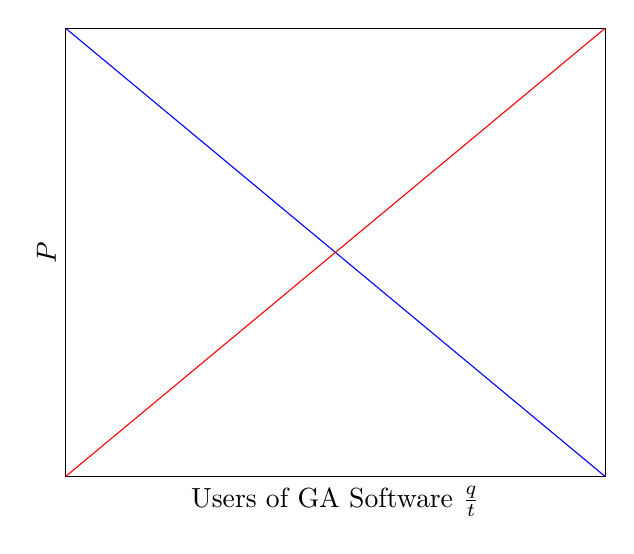
\begin{tikzpicture}
    \begin{axis}[
    domain=0:3,
    xmin=0,
    xmax=2,
    ymin=0,
    ymax=2,
    xlabel={Users of GA Software $\frac{q}{t}$},
    ylabel={$P$},
    ticks=none,
    samples=50,
    smooth,
    no markers,
    ]
    \addplot {2 - x};
    \addplot {x};
  \end{axis}
\end{tikzpicture}

\hfill \\
As the price of a substitute and compliment increase (in this case, a CFI), we expect the demand of our product to increase, causing our demand to increase at any price point and thus causing our curve to shift right as such:  

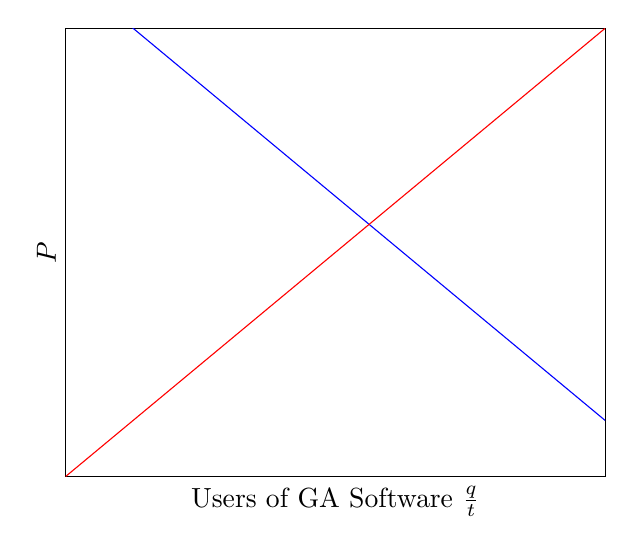
\begin{tikzpicture}
  \begin{axis}[
    domain=0:3,
    xmin=0,
    xmax=2,
    ymin=0,
    ymax=2,
    xlabel={Users of GA Software $\frac{q}{t}$},
    ylabel={$P$},
    ticks=none,
    samples=50,
    smooth,
    no markers,
    ]
    \addplot {2.25 - x};
    \addplot {x};
  \end{axis}
\end{tikzpicture}

\item
If we see an increase in our capacity to serve clients (e.g. a server upgrade to allow for more users and faster response time), we would expect more supply for a given price point, causing a right shift. 

\begin{tikzpicture}
  \begin{axis}[
    domain=0:3,
    xmin=0,
    xmax=2,
    ymin=0,
    ymax=2,
    xlabel={Users of GA Software $\frac{q}{t}$},
    ylabel={$P$},
    ticks=none,
    samples=50,
    smooth,
    no markers,
    ]
    \addplot {2.25 - x};
    \addplot {x - 0.25};
  \end{axis}
\end{tikzpicture}

\item
    A change in quantity supplied will not imply a change in supply. If you think about the number of iPhones being produced right now, it is possible that Apple over produced the quantity the supply, whereas the quantity supplied is not the same as the minimum supply needed to reach equilibrium. Conversely, if the supply changes, that does imply that quantity supplied will change. This is because the quantity supplied must meet supply on the graph to reach equilibrium. 

\item
    A good example of a 'dual shift' problem with regards to my CTM would be if we have another institution that wants to use our software, and supply of additional servers for us to use increases. This means that the demand for out product will increase. Below is a graph of what models for this would look like (here supply is represented in black): \\

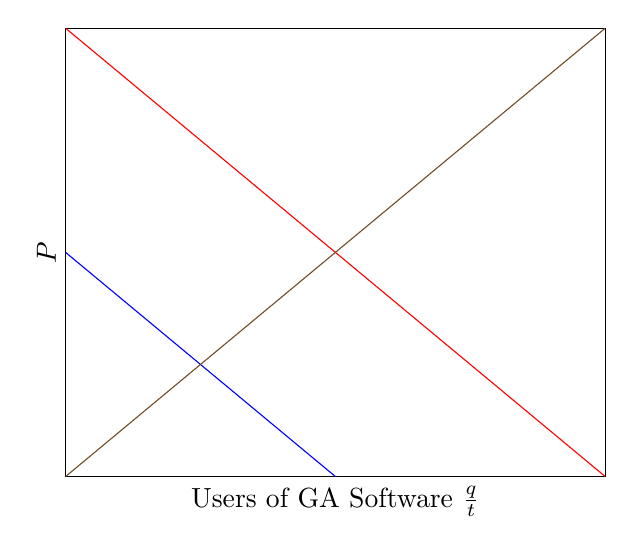
\begin{tikzpicture}
  \begin{axis}[
    domain=0:3,
    xmin=0,
    xmax=2,
    ymin=0,
    ymax=2,
    xlabel={Users of GA Software $\frac{q}{t}$},
    ylabel={$P$},
    ticks=none,
    samples=50,
    smooth,
    no markers,
    ]
    \addplot {1 - x};
    \addplot {2 - x};
    \addplot {x};
  \end{axis}
\end{tikzpicture}

\hfill \\
If we take a look at case II, where supply changes, we see an effect where the price of equilibrium decreases. 

    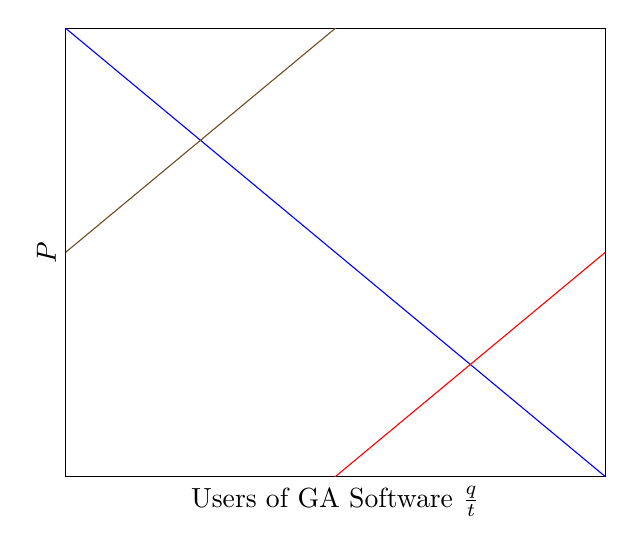
\begin{tikzpicture}
    \begin{axis}[
    domain=0:3,
    xmin=0,
    xmax=2,
    ymin=0,
    ymax=2,
    xlabel={Users of GA Software $\frac{q}{t}$},
    ylabel={$P$},
    ticks=none,
    samples=50,
    smooth,
    no markers,
    ]
    \addplot {2 - x};
    \addplot {x-1};
    \addplot {x+1};
  \end{axis}
\end{tikzpicture}

Without more information, we cannot tell if our equilibrium price will increase or decrease when we take both of these graphs into account.


\end{enumerate}




\end{document}
